\textbf{COLUNI 2021 -- Questão 37}\par\medskip Analise o texto e a imagem abaixo:

\par

Primeira República brasileira é um período marcado por grandes contrastes. Ao mesmo tempo em que é possível notar uma grande euforia com relação às novas tecnologias, à civilização, ao progresso e à modernidade, é um momento marcado também pelos efeitos menos positivos das mudanças que foram empreendidas por agentes políticos e seus impactos na vida de milhares de pessoas. Dentre diversos movimentos sociais ocorridos nesse momento, pode-se citar a Revolta da Vacina ocorrida no Rio de Janeiro em 1904, como resultado da reação da população do Rio de Janeiro às ações de modernização, remodelação urbana e medidas sanitaristas levadas a cabo por seus governantes e outras autoridades, dentre as quais se destaca o médico sanitarista Oswaldo Cruz.

% COLUNI-AUTO-FIGURES-BEGIN
\begin{figure}[htbp]
\centering
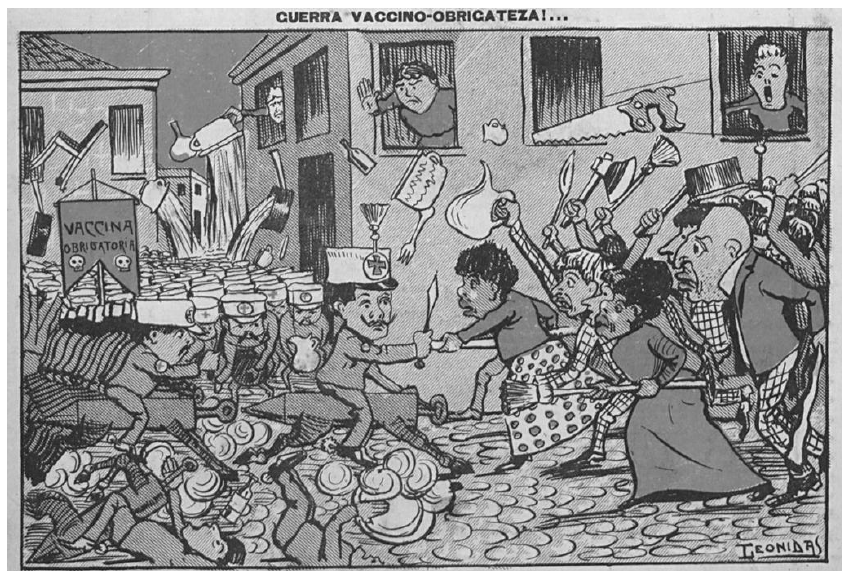
\includegraphics[width=0.95\linewidth]{static/simulados/coluni/figuras/2021/questao-37/figura-1.png}
\end{figure}
% COLUNI-AUTO-FIGURES-END

“Espectaculo para breve nas ruas desta cidade: Oswaldo Cruz, o Napoleão da seringa e lanceta, à frente das suas forças obrigatórias, será recebido e manifestado com denodo pela população. O interessante dos combates deixará a perder de vista o das batalhas de flores e o da guerra russo-japonesa. E veremos no fim da festa quem será o vaccionador à força!” Disponível em: http//memoria.bn.br/docreader/docreader.aspx?bib=116300\&pesq\&pagfis=3567. Acesso em: 12 jan. 2021.

\par

Com relação à Revolta da Vacina, analise as afirmativas abaixo:

\par

I. A defesa da salubridade urbana e da modernização da cidade, promovida pelas autoridades, possibilitou a instalação de uma campanha de saneamento e de vacinação obrigatória contra a varíola. II. A população foi informada da importância da vacinação a partir de uma ampla campanha de esclarecimento conduzida por órgãos governamentais e divulgada por meio de jornais e revistas. III. O descontentamento com as reformas urbanas, a impopularidade do governo e a obrigatoriedade da vacinação provocaram o desencadeamento de uma revolta popular na cidade do Rio de Janeiro.

\par

Está CORRETO o que se afirma em:

\begin{enumerate}
\item I, II e III.
\item I e II, apenas.
\item II, apenas.
\item I e III, apenas.\end{enumerate}
